% File name: GF2/Reports/Andy_Final_Report/Andy_Software_Final_Report.tex
% Final Report for Software project.
% Author: adh
% Date: Wed 05 Jun 2013 23:33

\documentclass[a4paper,10pt]{article}  % Standard document class
\usepackage[english]{babel}            % Set document language
\usepackage{fullpage}                  % Set up page for small margins etc

\usepackage{graphicx}                  % For including images in document
\usepackage{placeins}                  % Allows use of \FloatBarrier
% to avoid images or tables
% moving into next section
\usepackage{subfig}                    % For subfigures...

\usepackage{amsmath}                   % For improving maths/formula typesetting
\usepackage{tabularx}                  % Table changing package

\usepackage{algpseudocode}             % For producing algorithms/flowcharts
\usepackage{listings}                  % For including source code in document

\usepackage{color}
\definecolor{grey}{rgb}{0.5,0.5,0.5}

\usepackage{listings}                  % For including source code in document
\lstset{
  basicstyle = \footnotesize\ttfamily,
  commentstyle = \color{grey},
  keepspaces = true,
  keywordstyle = \color{blue},
  language = C++,
  numbers = left,
  numbersep=5pt,
  numberstyle=\tiny\color{grey},
  stepnumber=5,
  tabsize=2,
}


% Provide command for scientific notation
\providecommand{\e}[1]{\ensuremath{\times10^{#1}}}
\providecommand{\degrees}{\ensuremath{^{\circ}}}

% Define title here:
\title{Project GF2: Software\\ Second Interim Report\\ Software Design
  Team 1}
\author{George Ayris\\ gdwa2\\ Emmanuel \\ Parser \& Scanner
  \and James Glanville\\ jg597\\ Emmanuel \\ Scanner \& Parser
  \and \textbf{Andrew Holt}\\ \textbf{ah635}\\ \textbf{Emmanuel}\\ \textbf{GUI}}
\date{06 June 2013}

\begin{document}

% generate title
\maketitle
\vspace{\stretch{1}}
\tableofcontents
\newpage

\section{System Overview}
\label{sec:system-overview}

\subsection{Logic Simulator}
\label{sec:logic-simulator}

A logic simulation package has been developed, allowing a user to
define a logic circuit using a specialised, custom designed definition
language and to run this circuit in a simulation, observing the output
at various points in the circuit. The circuit may be run for a number
of cycles, selected by the user. The simulation may then be run for
some further cycles, or restarted from scratch. There is also an
option to run the circuit continually, observing the output in a
scrolling fashion.

The user may interactively set the value of any switches defined in
the specification value and observe the effect of this change in the
circuit as it continues to run.

If the user decides they would like to observe the signal at a point
previously un-monitored, they may add a new monitor to the circuit. To
avoid too many monitors being displayed together and causing
difficulty in reading the traces, a monitor may also be removed from
the circuit.

The definition file is selected from a file select dialog, allowing
multiple circuits to be tested during a single session.

The logic simulator provides helpful text output at the bottom of the
screen to warn the user of errors and keep track of how many simulations
have been run.

\subsection{Software Structure}
\label{sec:software-structure}

The software is structured across a number of files in the
\texttt{src} directory. The main file is \texttt{logsim.cc}, which sets
up the simulation package and calls the classes in the other files as
required.

When a new file is loaded, it is scanned and parsed, using objects
derived from the \texttt{scanner.cc} and \texttt{parser.cc} files
respectively. If the parsing is successful (the definition file
contains no errors), the circuit is created using classes in the
\texttt{devices.cc}, \texttt{devicetable.cc}, \texttt{monitor.cc},
\texttt{names.cc} and \texttt{network.cc} classes. Each of these files
defines a class of the same name to deal with a different part of the logic
simulator. There is also a header file (\texttt{filename.h}) which
contains class definitions; function prototypes; and variable and type
definitions for each of the classes.

\texttt{devices.cc} deals with the creation of different
devices in the circuit and the specification of these devices
(e.g. the number of inputs), along with setting the values of switches
and calculating the output of each device for a clock cycle of the circuit.

\texttt{devicetable.cc} defines a data type for associating the
devices with more meaningful names, so that the devices may be more
easily access.

\texttt{monitor.cc} deals with the monitors in the circuit: creation
and removal of monitors, as well as giving the signal level of each
monitor point at each clock cycle.

\texttt{names.cc} translates between the internal representation of
each component through an \texttt{id} and the more user friendly name
given to each device, monitor, switch or clock.

\texttt{network.cc} manages the network of devices and components by
creating the device outputs as required and defining the connections
between device outputs and inputs.

The final file required is \texttt{gui.cc}, which operates the user
interface. This is created using wxWidgets, a cross platform gui
toolkit. The \texttt{MyFrame} class creates the gui and handles user
interaction events and the drawing of the traces. It can make
modifications to the circuit as the user specifies using the graphical
options.

The whole project follows the object oriented programming
methodology. This means that the code is very modular, and the
different classes are not dependant on the other ones. For example, a
completely different interface could be developed and use the same
back-end software. Equally, a different parser could be implemented
and, provided all the features were implemented in some way or
another, the whole system would be identical to anyone not looking
inside the parser class.

This methodology is ideal for multi-programmer projects such as this
as it allows independent development of different classes with no
detailed knowledge of how the other programmers are designing and
implementing the internals of the other classes.

\section{Teamwork Overview}
\label{sec:teamwork-overview}

The teamwork was organised such that James would lead development of
the scanner and lead testing of the parser. George would lead
development of the parser and testing of the scanner. I was
responsible for the gui programming.

This setup worked well for the first stage of the project, allowing
each of us to become familiar with a different aspect of the
program. A downside of this was that it was difficult to talk through
design decisions with each other since our experience and growing
expertise for the project lay in different areas. It is often very
helpful to talk through the suggested design before implementing it as
it both clarifies in your own mind as you explain it and often the
other person will think about some unconsidered problem. However,
since I know almost nothing about how the parser operates, and
similarly George knows little about the GUI code, it is very hard to
properly discuss what we are doing.

When the maintenance task was released, each of us took on one of the
new tasks. This system worked well, each new task corresponded loosely
to the original split of the system development.

\section{Software Development}
\label{sec:software-development}

As the lead developer on the graphical user interface (gui), the
majority of my software development has been associated with
\texttt{gui.cc} and its header file. These define the classes used by
wxWidgets to create the application user interface and handle the
graphics used to draw the traces. The \texttt{MyGLCanvas} class is
derived from the \texttt{wxGLCanvas} class, which creates an area to
be drawn in using OpenGL. This class has undergone fairly minor
changes from what was provided. The \texttt{MyFrame} class is derived
from the \texttt{wxFrame} class. There is a slight difference between
the terminology used in wxWidgets and general computer speak, in that
usually a window refers to an area of the screen which displays the
interface for a particular program or application and is controlled by
the operating system's window manager. In wxWidgets, this is referred
to as a frame, and a window may control the display in a part of the
frame (for example the scrollable section containing the traces is a
window in wxWidgets speak).

In order to add an element to the wxWidgets frame, the element must be
defined in the \texttt{MyFrame} class constructor and given an
\texttt{ID} which is defined in an \texttt{enum}. For the new element
to perform a useful function when the user interacts with it, it must
be linked to a call-back function using the event table.

\subsection{MyFrame Development}

The main task of developing the gui was to create a user interface to
meet the specifications, while also being intuitive to use and
aesthetically pleasing. One particular design decision I made early on
was that because the program was to perform a fairly limited set of
functions, these should all be immediately accessible to the user
without a need for using the menu bar. Each function would therefore
have a widget on the gui.

For the structure of the user interface, it was decided to have the
window in a vertical orientation, with the user controls at the top,
trace displays in the middle and a message box to give the user
feedback and useful information at the bottom. This is reflected in
the final design (see figure \ref{fig:guiss}).
\begin{figure}[!htb]
  \begin{center}
    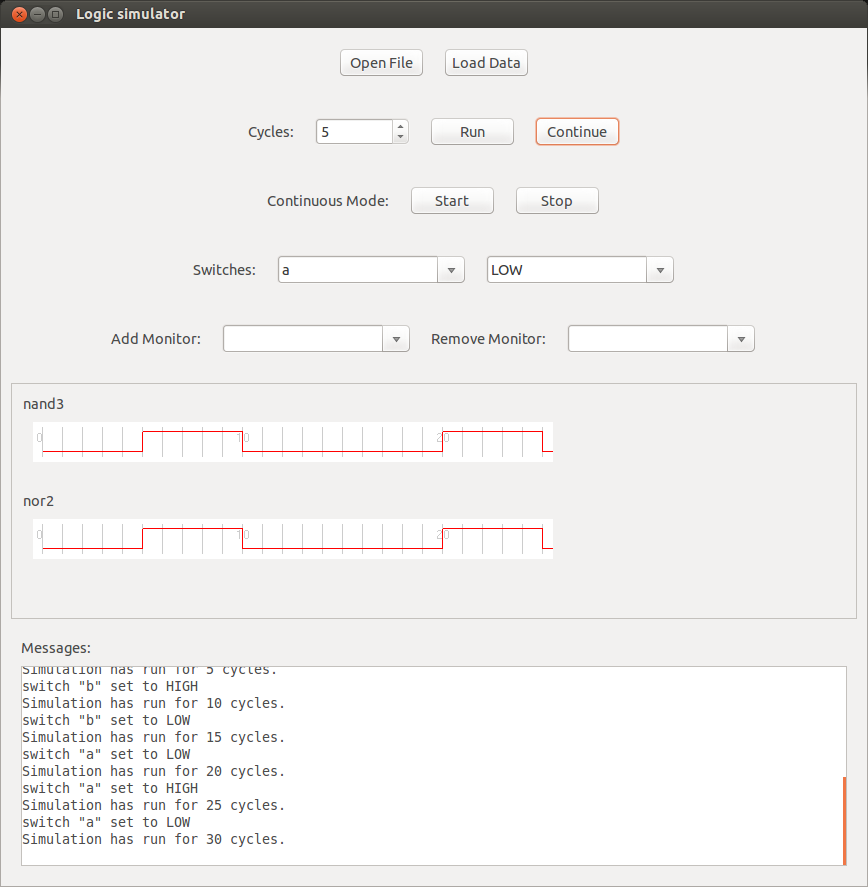
\includegraphics[width=0.8\textwidth]{GUI_Screenshot.png}
  \end{center}
  \caption{Screenshot of graphical user interface running under Ubuntu
  Unity.}
  \label{fig:guiss}
\end{figure}

This design was achieved by using a vertical box sizer as the top
level sizer for the display. The controls for each different function
provided are grouped together into a single row on the interface. For
example, the top row of controls contains buttons for selecting and
loading a definition file from the computer filesystem. The bottom row
provides options for adding and removing monitors to the trace
options. This is implemented by creating a horizontal box sizer for
each set of controls and placing this sizer into the top sizer. While
this design works and is fairly intuitive, it is not particularly
aesthetically pleasing. More detailed planning at the beginning of the
project would have helped to create a nicer interface.

In order to set a switch value, it is necessary to select both the
switch to be set and the value required to be set to. This is not a
very neat way of setting a switch and does not provide a good metaphor
for the actual process of switching. However this method was used as
the software back-end provides no way of accessing the current value
of the switch setting. It is thought that a function could be provided
in the devices class to return the value of a given switch. Since the
menu drop down method worked, it was decided to focus efforts on other
areas before coming back to improve this.

There was initially some confusion over the specification for adding
monitors in the user interface. Since monitors are defined in the
specification file, I took ``add the specified output signal to the
current list of monitor points'' to mean that there were two types of
monitor: a displayed monitor and a hidden monitor. The add and remove
monitor functions were therefore to change the state of a defined
monitor from the hidden list to the displayed list and
vice-versa. This method would require the user to define any points
they would like to look at in the specification file, but not force
them to display all of these points at once. I support this design
method as it highly encourages the user to think fully about the
circuit before stepping into the simulation, considering what might go
wrong with their circuit and so which points may be useful to monitor
\emph{before} jumping into the simulation package. This would also
allow the user to define a large number of possible monitor points
(each given an obvious and intuitive name), but only select the
relevant traces for viewing at a particular time, ensuring clarity of
the traces which are shown. While I believe that my interpretation of
the brief encouraged good design for these reasons, it came to light
during the initial demonstration that the required functionality was
to define a new monitor point and display it. During the final week of
the project, the task of fixing this was assigned to another team
member as there was a lot to be done for the gui and this task didn't
require much experience with wxWidgets. At the time of writing, the
functionality to add a new monitor point has been implemented, but the
monitor points defined in the specification file has been lost. This
should not be too hard to fix since the code previously did this well,
however this has not been prioritised in the closing stages of the
project.

The most difficult and time consuming part of the gui development was
the display of the traces. The standard method, and that in the
supplied code, was to use a single GLCanvas to display all the traces,
and allow the GL rendering code to format and display the appropriate
traces. This design, however, doesn't create a consistent interface
with the rest of the application and other applications as the OpenGL
graphics look very different to the graphical elements defined by the
wxWidgets toolkit. Since consistency is one of the primary elements of
an intuitive and well designed gui, it was decided to use a method
which simplified the OpenGL drawing and used wxWidgets for the
organisation and display of multiple traces.

For a single trace, the required elements were a \texttt{wxStaticText}
object to display the name of the trace, and a \texttt{MyGLCanvas}
object to display the actual trace. These were to be grouped together
in a horizontal sizer. To allow multiple of these traces to be
displayed and flexibility of which monitor was displayed in which,
\texttt{vector}s were used to contain each trace. The different traces
(in the vectors) were then added to a vertical sizer to hold all the
traces within a scrolling window. The different vector elements may be
easily hidden and shown to ensure that only traces actually required
are shown.

While this method works well and is highly flexible, there are a few
issues. Primary among these is that the traces were not aligned with
one another on the x-axis. This was overcome by putting the trace name
above the trace, instead of to the left. Given more time, a better
solution would be to use a grid sizer. This would allow the alignment
of the traces, while simultaneously allowing arbitrarily long trace
names. Grid sizers also allow easy hide and show functionality of
single rows, so this could replace the current functionality of the
vector of horizontal sizers. The vector of canvases would remain
useful as this allows display of an arbitrary trace in each row, so
the monitors may be reordered as required by the user.

This provides a good example of one of the major difficulties faced in
the gui design. While it is always useful to come up with a detailed
design of the system \emph{before} beginning the implementation, I
didn't know anything of how wxWidgets worked, what it could do and
what its limitations were. It was therefore very difficult to come up
with a good and meaningful design. As I've learned many of the
wxWidgets ways of thinking and doing things over the course of the
project, I now feel that I could come up with a far superior initial
plan, and would plan to do the traces with a grid sizer (now that I
know of its existence).

A particular challenge of the method I selected for displaying the
traces was scrolling. After a large amount of trial, error and reading
examples online, vertical scrolling was implemented using the
\texttt{wxScrolledWindow} type. This allows the user to display more
traces than can fit on the display at a time, and scroll among
them. This was working well until two days before the hand
in\footnote{as seen in the code run by Tim Love 04/06/2013.}. However,
at the time of writing, this function seems to have been broken during
the same commit as stopped the defined monitors from being
displayed. This may or may not be fixed before the final hand in.

Horizontal scrolling of the window to display traces longer than the
size of the frame has proved far more difficult. It is not clear why
wxWidgets does not do this automatically as with the vertical
scrolling. However, there do seem to be issues with the way sizers and
canvases interact, and the sizers do not become aware of the size of
the canvas as it changes. This seems to mean that the sizer always
thinks the canvas can fit on the screen and no scrollbar is required
for the horizontal direction. Much investigation has been carried out
in this to no avail, it seems that scrolling and OpenGL canvases just
don't play well together. To fix this, manual scrolling could be
implemented, however this would need some fairly serious time
investment which was not possible at this stage of the project.

The message box at the bottom of the gui is a more successful story
than the trace displays. This is implemented using a read only,
multiline \texttt{wxTextCtrl}. Along with the
\texttt{wxStreamToTextRedirector}, this allows messages to be printed
to the gui instead of to stdout. One particular challenge in this was
displaying the error messages properly. The error messages are
formatted to display a carat (\verb+^+) under the symbol which is
causing the error. However, by default the \texttt{wxTextCtrl} uses a
variable width font. This caused the carat to be displayed in the
wrong place. This was overcome by changing the font to a fixed width
font. Font selection turned out to be a non-trivial problem, however
the documentation of \texttt{wxFont} eventually led to a working
solution.

\subsection{MyGLCanvas Development}

Far less modification was required to the given \texttt{MyGLCanvas}
class, however a few modifications were made.

The \texttt{Render} method of the class was modified. While the
original \texttt{Render} function was to display all the traces, the
modified version should display only a single monitor trace. It is
therefore called with two arguments, one which selects the monitor to
be displayed in that particular canvas, and the other to set the
number of cycles to be displayed.

X-ticks have also been added to mark the clock transitions, and every
tenth transition is marked with a number to display the number of
cycles up to that point.

The functions to control mouse interaction or display particular text
on the canvas have been disabled/removed.

There is a major bug in the rendering of the traces
which has not yet been resolved. It was found that often the trace is
not displayed properly, and despite the correct \texttt{y} values been
shown in the text output, the trace is not drawn in the correct
place. It appears that for some, yet unknown, reason, the trace
attempts to be redrawn after display but without the correct trace
being shown. It has been found that if the line \texttt{Render();} in
function \texttt{MyGLCanvas::OnPaint} (line 185 in \texttt{gui.cc}) is
removed, the display works correctly. However, this line is required
for redrawing the traces when the window is resized. The cause behind
this has not yet been established, so currently there is a decision to
be made between showing wrong traces and not redrawing the traces when
the window is resized. Changing the inclusion of this line verifies
that both aspects of the program work, just unfortuantely not at the
same time!

\subsection{Continuous Display Mode}

The maintenance phase of the development required the addition of a
continuous display mode, where the display scrolls in the manner of an
oscilloscope type trace.

In order to implement this, new versions of the \texttt{MyFrame::runnetwork}
and \texttt{MyFrame::Render} methods were created. Each would
increment the displayed trace by 1 and display only the previous 10
traces.

In order to continuously update the display, pressing the ``Start''
button begins a \texttt{wxTimer}, which may be stopped by pressing
``Stop''. Every period (currently set to 500ms), the timer calls an
event. The event table then calls a callback function which calls the
updated \texttt{runnetwork} and \texttt{Render} functions to update
the display.

A screenshot of this functionality is shown in figure \ref{fig:contss}.
\begin{figure}[!htb]
  \begin{center}
    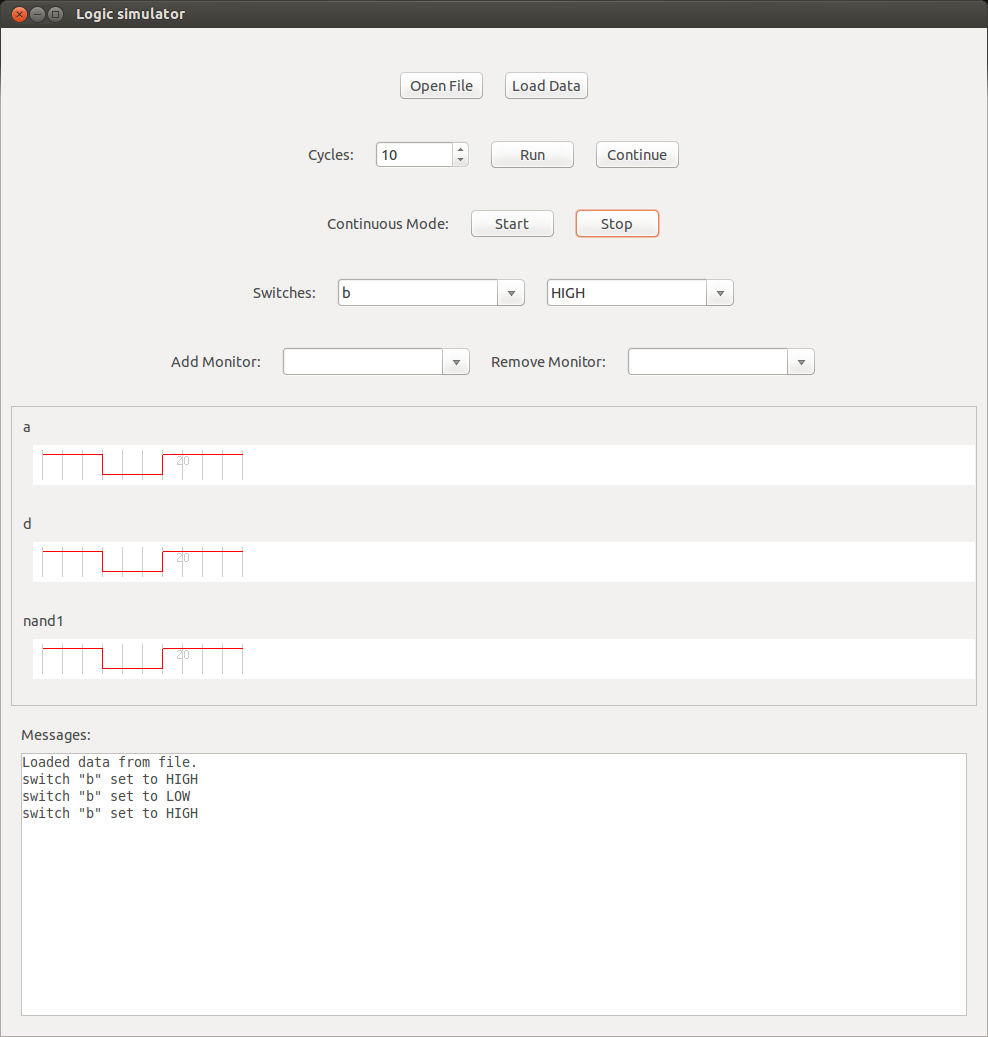
\includegraphics[width=0.8\textwidth]{Cont_screenshot.png}
  \end{center}
  \caption{Screenshot showing continuous mode operation}
  \label{fig:contss}
\end{figure}

\section{Test Procedures}
\label{sec:test-procedures}

For the gui, the only meaningful testing method was user testing. To
this end, I tested each feature as I implemented it, along with other
features which could have been broken by the new one. I also ensured
James and George were using the gui whenever possible so that they
could find bugs and issues that I may have missed.

Testing in the final stages showed many features to not work as
required. Some of these, like the monitor additions, had previously
worked, but stopped working when later features were added. The causes
of these have not been fully investigated at the time of
writing. Other problems, such as horizontal scrolling, have not been
fully implemented so testing of these was not possible.

\section{Known Bugs}
\label{sec:known-bugs}

I have outlined most of the known bugs relating the graphical user
interface as I have detailed the design and development. These all
apply at the time of writing but this does not guarantee that they
will not be fixed by the time of the hand in. This section is much
longer and the bugs far more serious than I'd like.
\begin{enumerate}
\item The defined monitors from the specification file do not appear
  in the monitors to add list as they should. This worked until the
  option to add monitors at any point in the circuit was implemented
  by another team member.
\item There are several issues with the scrolling window. It does not
  scroll horizontally due to issues with wx sizers and GL
  canvases. Vertical scrolling has also broken, at the same time as
  the monitor fault occurred.
\item It does not seem to be possible to allow resizing of the trace
  window at the same time as actually showing valid traces in the
  cavases, due to an issue with the \texttt{onPaint} function.
\item Sometimes the traces just aren't drawn as they should be. This
  is under investigation alongside the previous issue.
\end{enumerate}


\section{Conclusions and Further Work}
\label{sec:concl-furth-work}

Only a partially operating logic simulation system has been delivered,
and this would be unacceptable for a product release. One of the major
causes of this was a lack of proper planning at the beginning of the
project. Developers' lack of familiarity with the whole system also
cost us highly when all working on bug fixes in the closing stages.

I do think that the project was on a good trajectory until the final
week of the project, but there was too much left to do with
insufficient time at the end.

Given further development time, which would be necessary to deliver a
usable product, the following should be completed:
\begin{enumerate}
\item Develop a more intuitive method for setting switch values. This
  should provide a better metaphor for switching than the current
  system. This will require some gui modifications, but also back-end
  development to allow access to the current state of a switch.
\item The issues highlighted with the monitor points must be
  addressed. This would require investigating the changes to the
  relevant parts of the system in the last commit to break the
  software. The Git version control system that has been used
  throughout the project would make this fairly straightforward, but
  time has not been adequate to do this.
\item The method of displaying the traces in the scrolled window
  should be rewritten to make use of the more suitable grid sizer
  class. This would allow arbitrarily long names while ensuring
  correct alignment of the trace drawings.
\item The issues surrounding the scrolling problems should be
  thoroughly investigated and a solution found. This may involve a
  large increase in complexity of the user defined scrolling features
  instead of having wxWidgets take care of the scrolling.
\item The reason for the trace displays showing either the wrong trace
  or not resizing should also be thoroughly investigated and a
  solution found.
\item Further develop the continuous display mode to allow selection
  of both the speed and number of past cycles that are displayed.
\end{enumerate}
So far, neither students or demonstrators have found an adaquate
solution to the scrolling or trace display/resizing issues.

As a project, this has been challenging but enjoyable. It has been
very useful to gain experience of writing user interface software as
this is a very different ball game to any programming I had previously
done. While this has been a steep learning curve (clearly too steep
for me to deliver a working product in the time allowed), the skills
have already come in useful for my other project and probably will
continue to be useful in the future.

It has also been good to gain experience of programming in a team on a
larger project than I had previously done. It is in this setting that
the advantages of object oriented programming, version control systems
and other concepts from the 3F6 course have become apparent.

\appendix

\section{Software Listings}
\label{sec:software-listings}

\section{Example Circuits}
\label{sec:example-circuits}

\subsection{Logic Gate Array}

The first example test file defines a logic gate array. The circuit
diagram is shown in figure \ref{fig:testlgcct}.
\begin{figure}[!htb]
  \begin{center}
    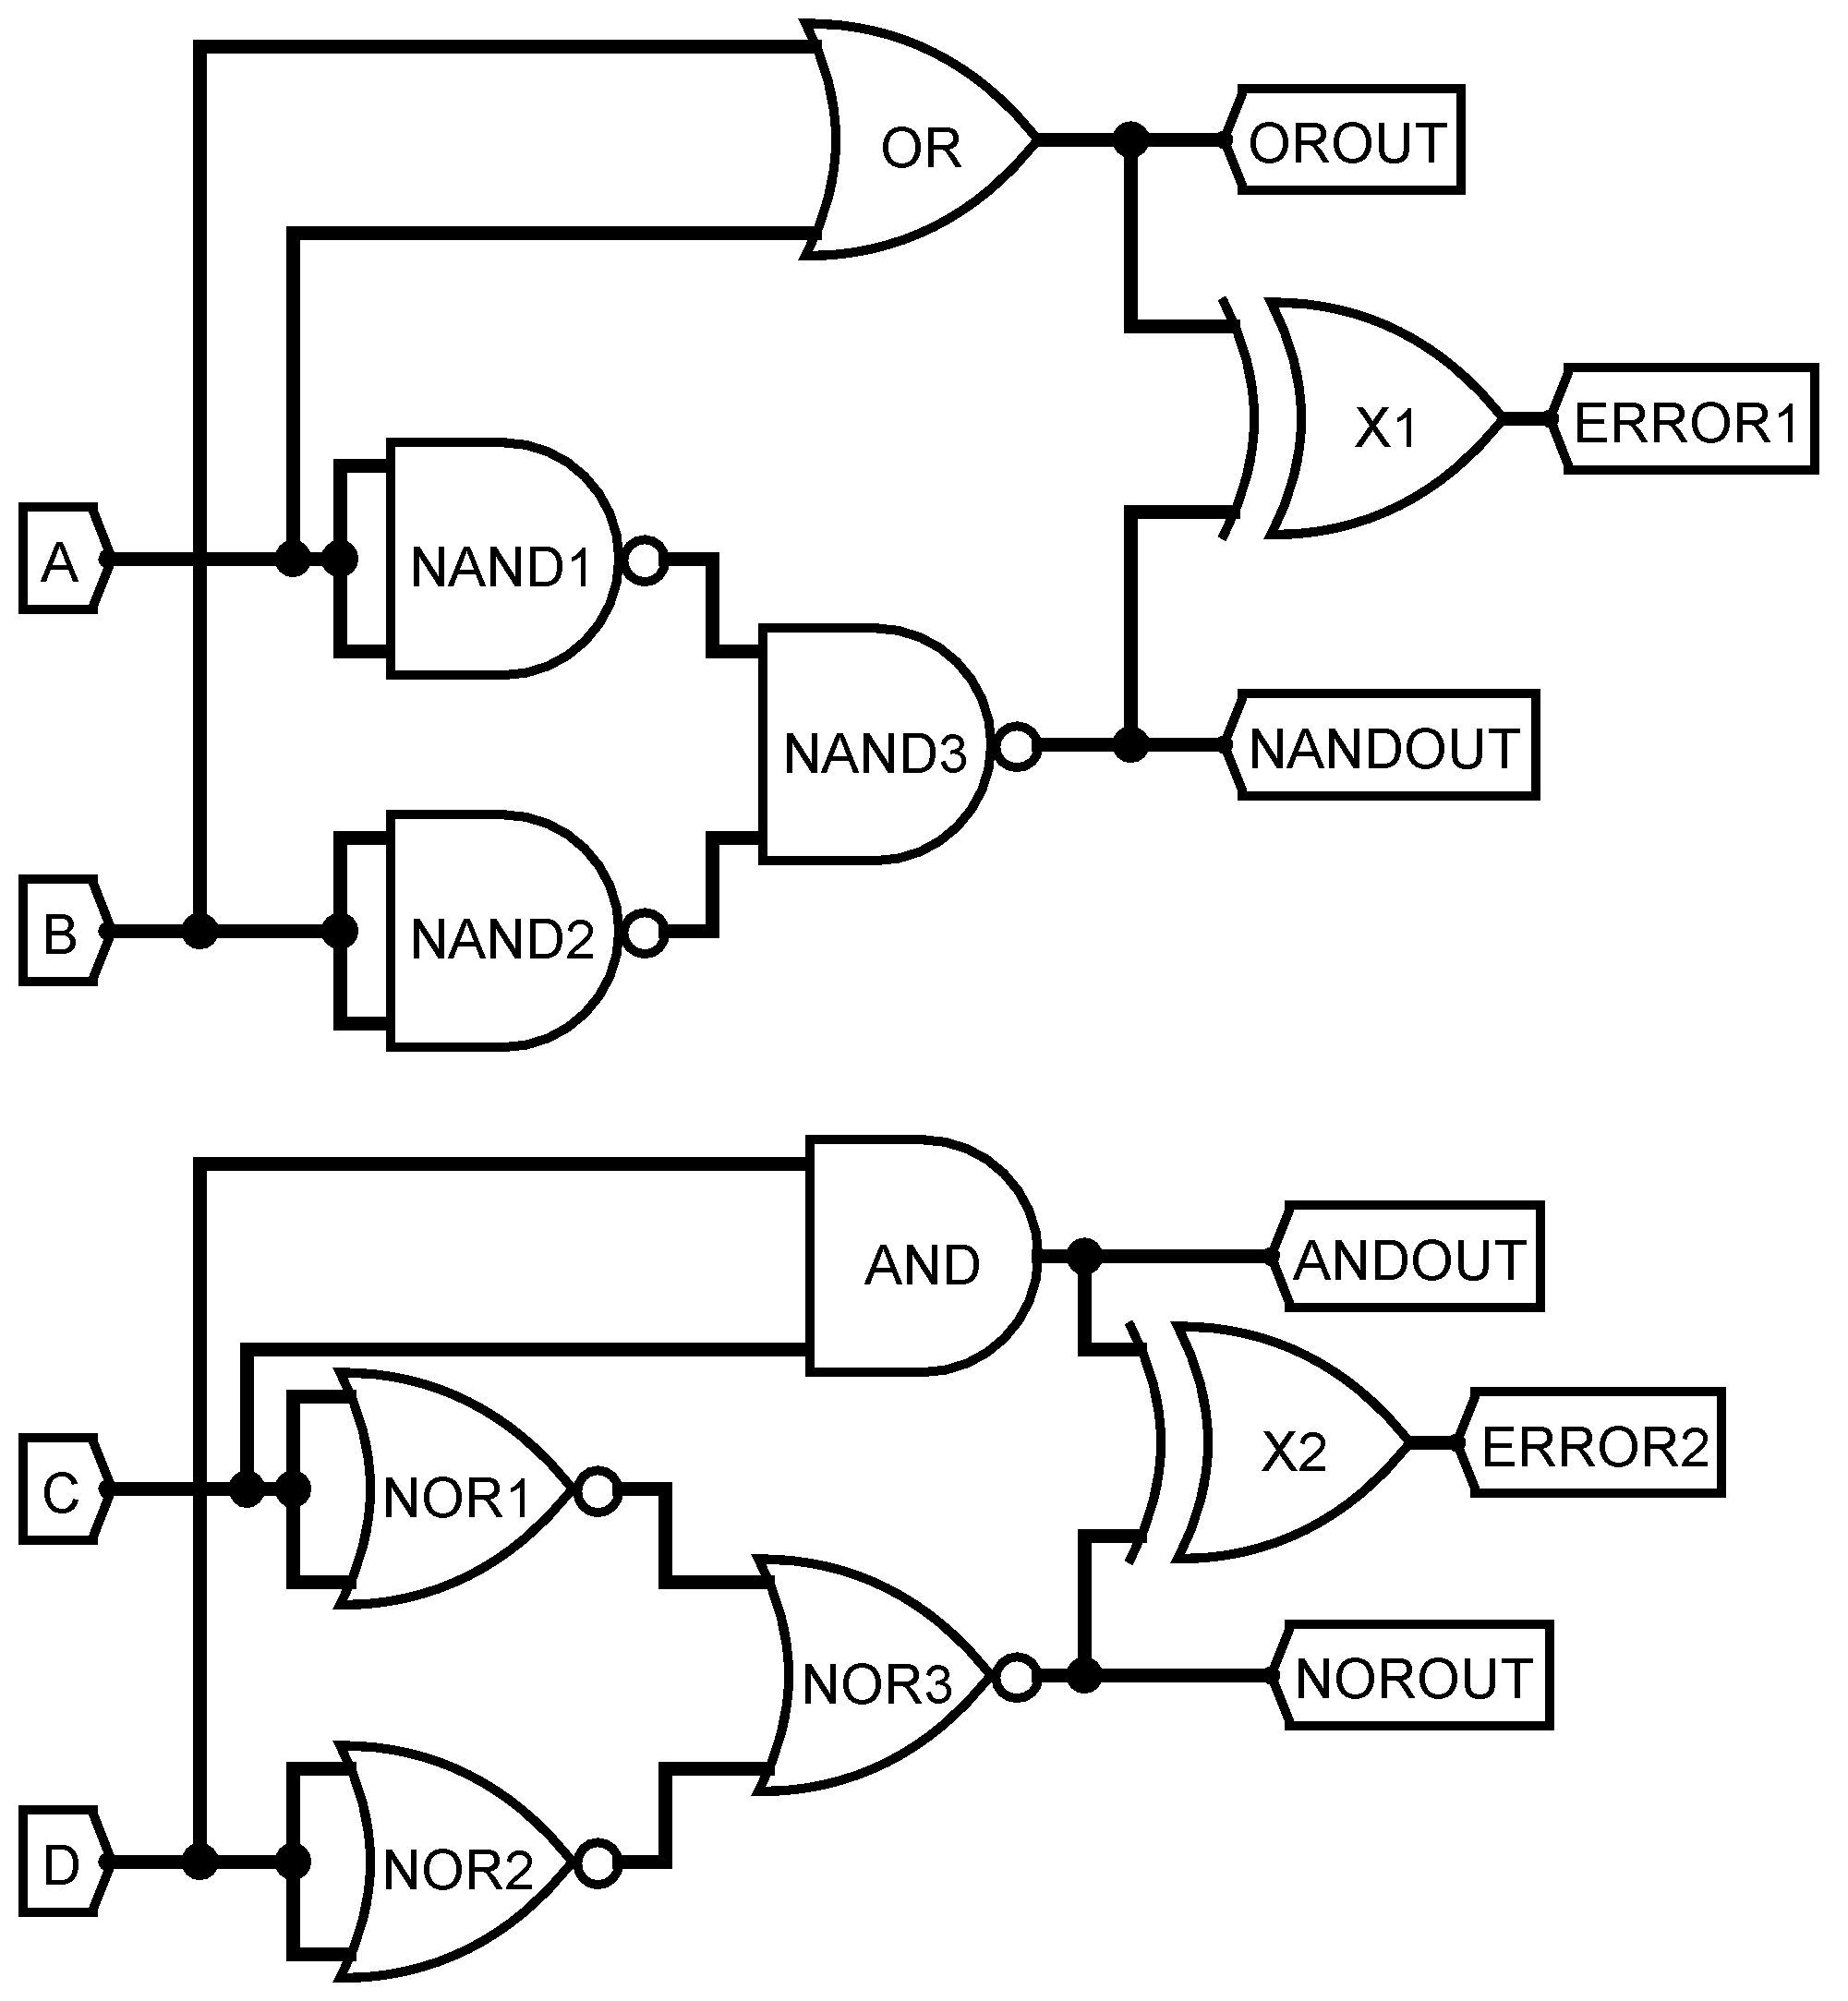
\includegraphics[width=0.6\textwidth]{testgates_schem.png}
  \end{center}
  \caption{Logic gate array test circuit.}
  \label{fig:testlgcct}
\end{figure}
This circuit is defined for the logic simulator using the following
definition file:
\lstinputlisting[language=VHDL,keywordstyle=\color{black}]{testgates.def}

The test result obtained from the logsim package is shown in figure \ref{fig:testlgss}.
\begin{figure}[!htb]
  \begin{center}
    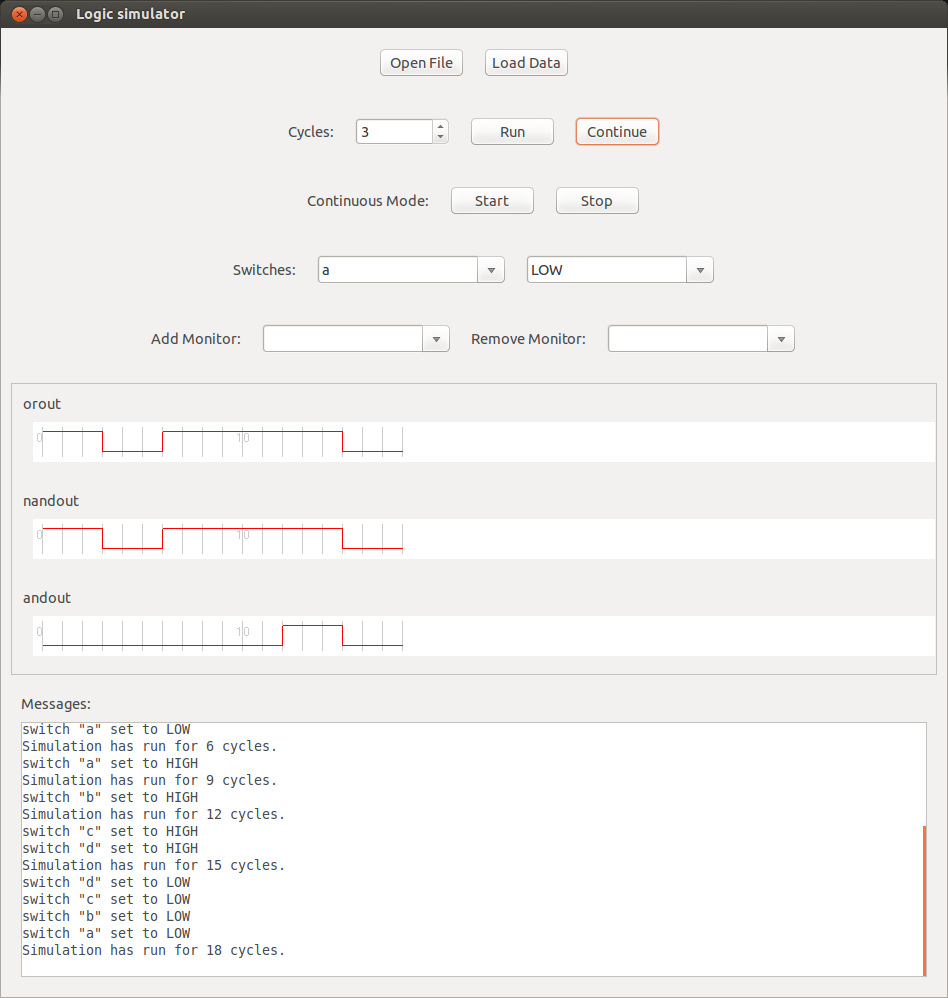
\includegraphics[width=0.8\textwidth]{testgates_screenshot.png}
  \end{center}
  \caption{Screenshot showing running of logic gate array test case.}
  \label{fig:testlgss}
\end{figure}
The outputs are correct according to the values of the switches set at
different points in the simulation.

\subsection{Shift Register}

A common sequential logic circuit is the shift register. It is
frequently used for driving a serial bus from a parallel device. The
circuit diagram is shown in figure \ref{fig:testsrcct}.
\begin{figure}[!htb]
  \begin{center}
    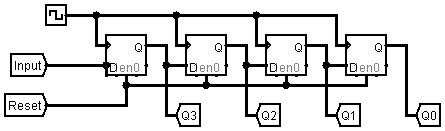
\includegraphics[width=0.8\textwidth]{shiftregister_schem.png}
  \end{center}
  \caption{Shift register test circuit.}
  \label{fig:testsrcct}
\end{figure}
The definition file is as follows:
\lstinputlisting[language=VHDL,keywordstyle=\color{black}]{shift_register.def}

The test result obtained from the logsim package is shown in figure
\ref{fig:testsrss}.
\begin{figure}[!htb]
  \begin{center}
    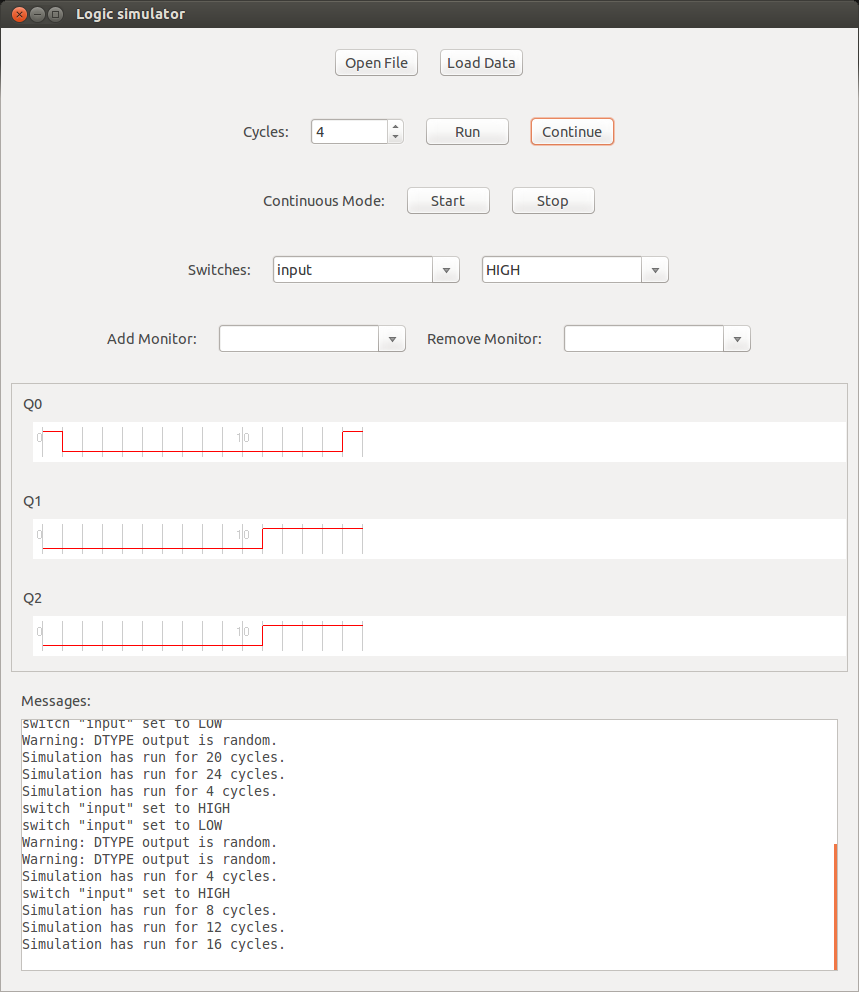
\includegraphics[width=0.8\textwidth]{shift_register_screenshot.png}
  \end{center}
  \caption{Screenshot showing running of shift register test case.}
  \label{fig:testsrss}
\end{figure}
The output shown does not correspond to the expected output. This is
due to the update to the d-type specification in the maintainance
phase, where the output of the gate is random due to the input changing.

\subsection{Signal Generator}

The final test case considered here displays the added functionality
from the maintainance case of the signal generator and the continuous
output mode. The circuit is a simply signal generator feeding an
inverter, as shown in figure \ref{fig:testsgcct}.
\begin{figure}[!htb]
  \begin{center}
    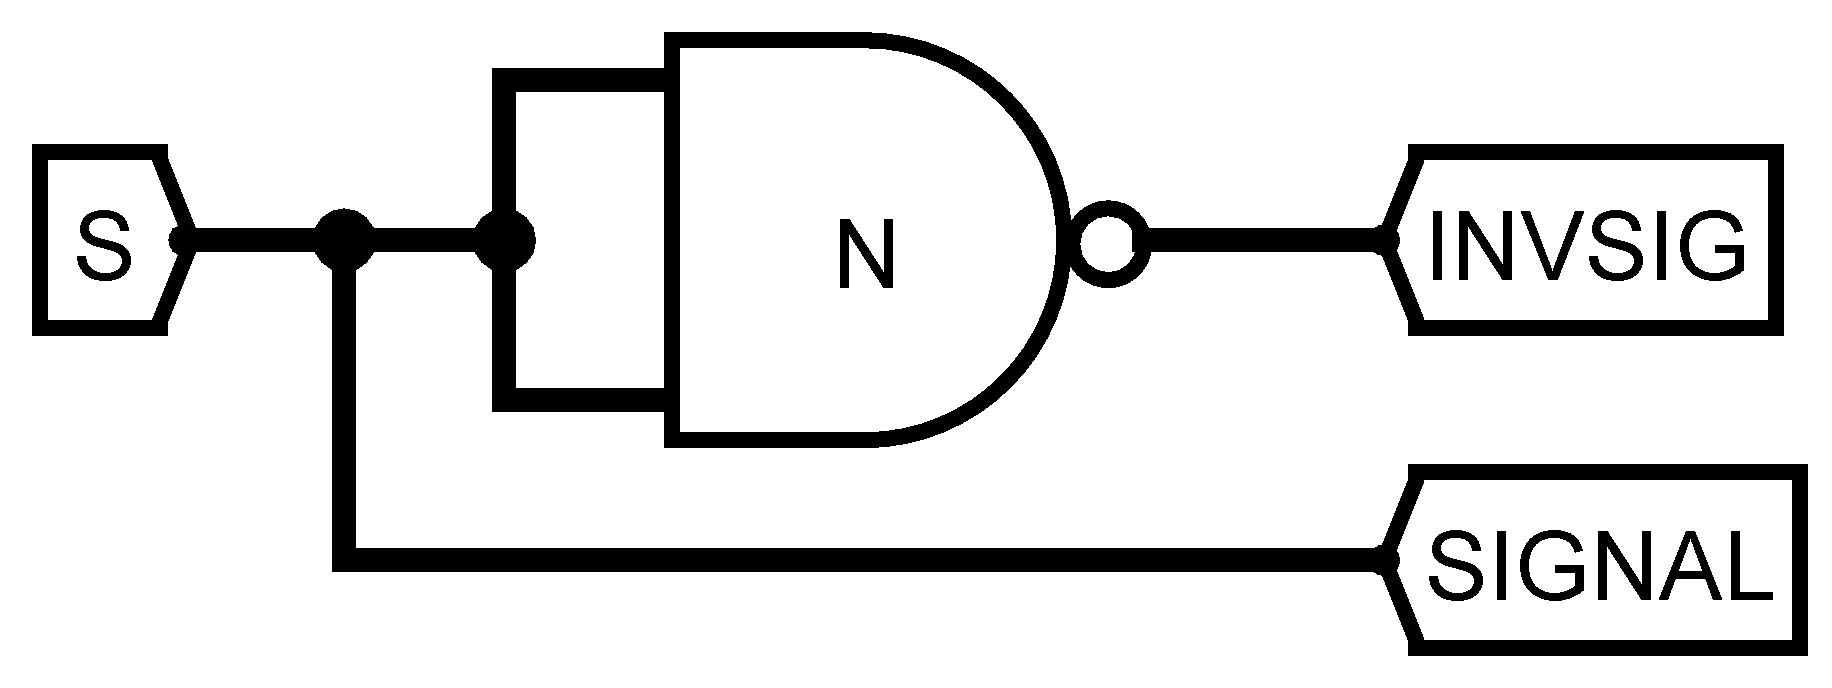
\includegraphics[width=0.8\textwidth]{siggen_schem.png}
  \end{center}
  \caption{Signal generator test circuit.}
  \label{fig:testsgcct}
\end{figure}
The definition file is:
\lstinputlisting[language=VHDL,keywordstyle=\color{black}]{siggen.def}

The test case is shown in figure \ref{fig:testsgss}.
\begin{figure}[!htb]
  \begin{center}
    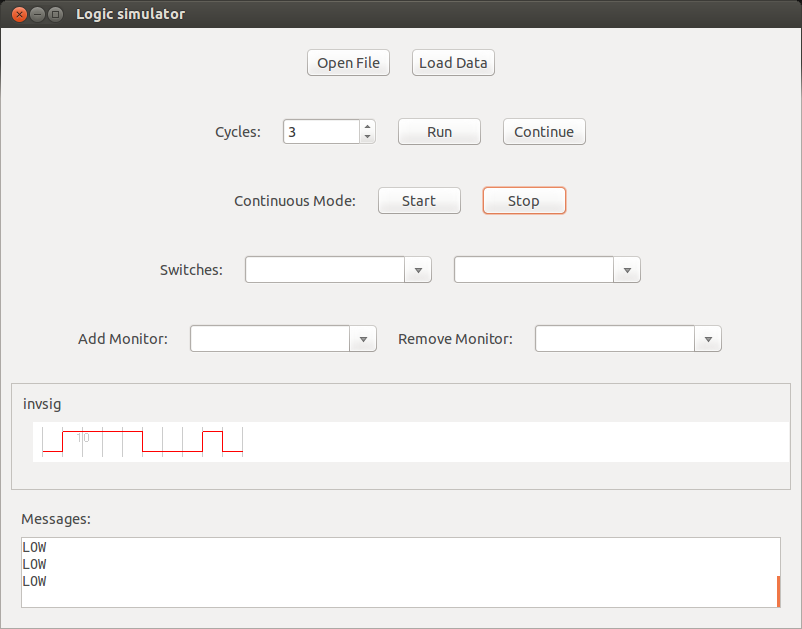
\includegraphics[width=0.8\textwidth]{siggen_screenshot.png}
  \end{center}
  \caption{Screenshot showing running of signal generator test case.}
  \label{fig:testsgss}
\end{figure}
The output can be seen to be the same as the inverted signal defined
in the definition file. The continuous mode is also seen to be
working, the tenth period is shown near the start of the trace.

\FloatBarrier
\section{Definition File Specification}
\label{sec:defin-file-spec}

The EBNF specification for the test definition case is:
\lstinputlisting{ebnf}


\section{System User Guide}
\label{sec:system-user-guide}

The user interface is shown in figure \ref{fig:ugimage}. Everything in
this guide apart from the starting of the program relates to
interaction with this screen.
\begin{figure}[!htb]
  \begin{center}
    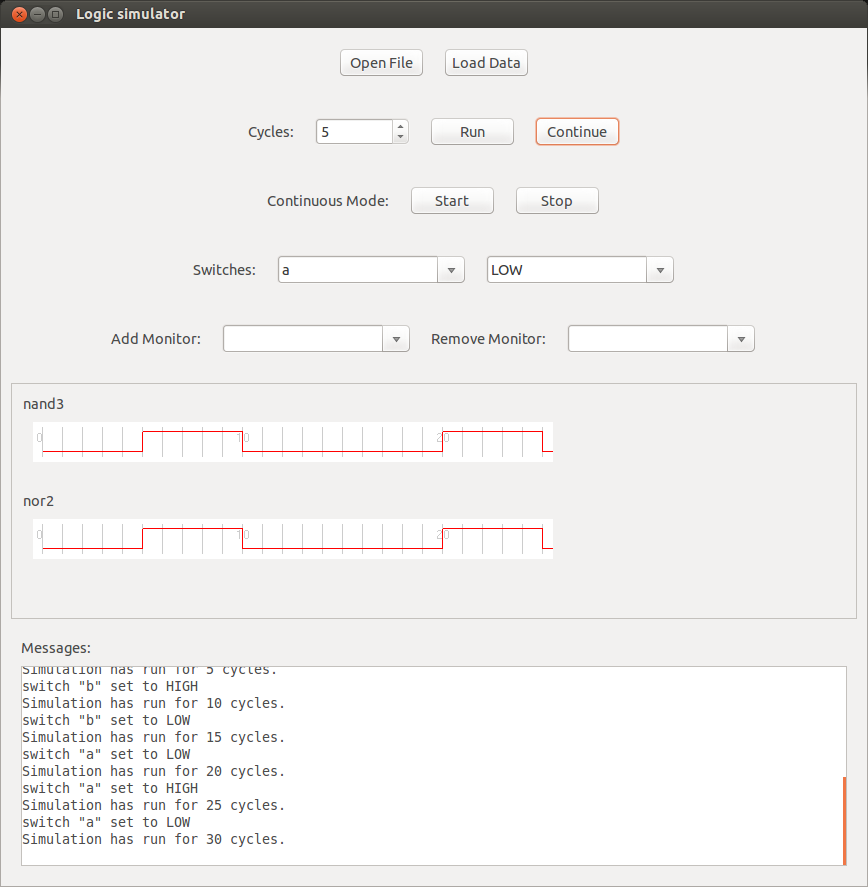
\includegraphics[width=0.8\textwidth]{GUI_Screenshot.png}
  \end{center}
  \caption{Main Screen on logic simulator.}
  \label{fig:ugimage}
\end{figure}

\subsection*{Starting the Program}

The logic simulation package may be run by running the command
\texttt{./logsim} in the directory of the compiled file. To load a
definition file, click on the \textbf{Open File} button. This will
bring up a standard file selection window. After selecting the desired
file, click \textbf{OK} to return to the main screen.

\subsection*{Definition Errors}

Any errors in the definition file will be highlighted in the message
display at the bottom of the program window. This will give detailed
information about the cause and location of the error, making
debugging fast and efficient. Once all errors have been corrected the
program may be run fully.

\subsection*{Setting up Monitors and Switches}

Once the definition file has been loaded, the \textbf{load} button
should be pressed. This populates the drop down menus with the
relevant devices for selection. To add a monitor point, simply select
the desired point from the list in the \textbf{add monitor}
drop-down menu, then enter a name for this monitor in the pop-up
window. They may be removed by selecting the monitor from the
\textbf{remove monitor} menu. To ensure all required information is
visible together, without many distracting and irrelevant output
traces, up to 10 monitors may be observed at once. The value of a
switch may be set at any time during the simulation by selecting the
desired switch from the \textbf{switches} drop-down menu, followed by
the level to be set from the \textbf{switch value} menu.

\subsection*{Running and Continuing the Simulation}

To run the simulation, simply select the number of clock cycles to
simulate in a single run (between 1 and 50), then press the
\textbf{run} button. The traces for all defined monitors will be
shown. The simulation may be \textbf{continued}, to observe the long
term behaviour or to investigate the effect of a changed switch level
on the circuit. The simulation may be run for up to 350 clock
cycles. If the simulation is run for a large number of cycles, the
traces may no longer be visible. In this case, simply drag the window
to become wider and the traces will increase in size so that more
clock cycles are visible.

\subsection*{Continuous Display Mode}

In order to run the circuit continually and observe the changing
signal levels, press the \textbf{Start} button. The monitors will show
the values for the 10 previous clock cycles in a continually updating
display until the \textbf{Stop} button is pressed.

\section{File Description}
\label{sec:file-description}

\end{document}